\chapter[Events for the Minimal Dark Matter model]{Event generation and reconstruction \mbox{for the Minimal Dark Matter Model}}

\lettrine{T}{}his chapter introduces the Minimal Dark Matter model in the context of the \mph analysis and describes all the steps made to generate Monte Carlo (MC) samples for this model. Reconstruction of objects in ATLAS from real events is also given.

\section{Non so se descrivere qui il minimal model}
Magari qui metto il paragrafo che ho scritto nel capitolo precedente riguardo il modello minimale. Cos\`i  spiego anche l'analisi \mph che mi serve per introdurre la generazione dei campioni.

\section{Model overview}
The Minimal Dark Matter (MDM) model, presented by Prof. Marco Cirelli\footnote{Institut de Physique Th\'eorique, CNRS, URA 2306 \& CEA/Saclay, F-91191 Gif-sur-Yvette, France}, extends the SM with a Electroweak (EW) fermion triplet, being a potential DM candidate~\cite{Cirelli:paper}. This particle ($\chi$) is triplet under $SU(2)_L$, where the subscript L indicates coupling only to left-handed fermions, and singlet under color and hypercharge ($Y=0$). Its relevant Lagrangian is very simple and reads:
\begin{equation}
\begin{split}
\mathcal{L}_\chi&=\frac{1}{2}\bar{\chi}\left(i\slashed{D}-M_\chi\right)\chi \\
			&= \frac{1}{2}\bar{\chi_0}\left(i\slashed{\partial}-M_{\chi_0}\right)\chi_0+\bar{\chi}^+\left(i\slashed{\partial}-M_{\chi^\pm}\right)\chi^+ \\
			&+ g \left(\bar{\chi}^+\gamma_\mu\chi^+\left(s_w A_\mu + c_w Z_\mu \right) +\bar{\chi}^+ \gamma_\mu\chi_0W^-_\mu + \bar{\chi_0}\gamma_\mu\chi^+W^+_\mu \right)
\end{split}
\end{equation}
where $g$ is the $SU(2)$ gauge coupling, and $s_w$ and $c_w$ are the sine and the cosine of the Weinberg angle.

All the possible interaction between $\chi$ and other SM particle are required to preserve the gauge and the symmetries of the SM particularly the lepton number. This constrain was not applied to an eventual 5-plet particle which would have been automatically stable anyway. On the other hand the triplet has important features even beyond the DM motivation and it is capable to be produced at collider rather than the 5-plet.

If one requires that $\chi$ is thermally produced via the freeze-out mechanism discussed in \Sect{\ref{sec:wimp}}, and that it constitues all the DM in the Univers, then we can extimate its mass to be \SI{3.0}{}$\div$\SI{3.2}{\tev}. This range of mass, of course, is out of reach from actual detectors. Nevertheless for masses lower than \SI{3}{\tev}, $\chi$ is a subdominant DM component if thermally produced and its existence is again well justified to pursue any search at colliders. So the Minimal model can be seen as a benchmark of the typical thermal-relic WIMP Dark Matter candidate, being a prototype for more complicated models, reproducing their low energy phenomenology with great accuracy.

As mentioned in the previous section, a way to search for WIMPs at colliders is via the so-called \emph{Mono-X} analyses. In this kind of searches the signal comes not only for the $\chi_0$ WIMP candidate particle but also from its two charged partners in the triplet. We can assume that the latter decay via a $\chi_0$ and soft, or low-momentum, charged pions (\pipm) both unreconstructed in a detector. 

A different, possible, scenario is that the tail of the decay distribution of the two charged $\chi$s might also leave tracks in the detector. These tracks would end when they decay as described into a couple of $\chi_0$ and charged pions. For that reason the \emph{disappearing tracks} would provide the most sensitive probe to the Minimal Model.

\smallskip
In this work a \mph analisys has been pursued following the lead of the one carried on in 2017 by the ATLAS Collaboration~\cite{paperMP}. In this context the \mph was re-interpreted and the Minimal Dark Matter model was tested by setting upper limits on pair of $\chi_0$ production.

In the \mph analysis, which is a cut\&count analysis (refer to Chapt. \ref{chapt:mph}, we are looking for a single high energy photon and large missing transverse momentum (\met) signature whose definition will be given in \Sect{\ref{sec:recoreal}}. Therefore it is characterized by a relative clean final state thanks also to a small set of SM processes that produces the same outcome. The minimal model predicts several way in which DM can be produced and revealed within a \mph analysis. Three examples of Feynman diagram are given in \Fig{\ref{fig:feynman}}.

 \begin{figure}[tp]
 \centering
 \begin{tikzpicture}
 [scale=0.5,decoration={
markings,% switch on markings
mark=% actually add a mark
at position .5  with {\arrow{>}}}]
 \draw[thick, postaction={decorate}] (-4,2) node at(-3,1)[above=2pt] {  $q$} -- (-2,0) ;
 \draw[thick, postaction={decorate}] (-2,0) -- (-4,-2) node at(-3,-1) [below=2pt] {  $\bar{q}$} ;
 \draw[thick,decorate,decoration={snake,amplitude=1.5mm,segment length=3.5mm}] (-2,0)--(1,0) node  at (-0.25,0) [below=3pt]{  $\gamma$,$\Zboson$};
 \draw[thick, postaction={decorate}] (1,0) -- (3,1) node at (2,0.5) [above]  {  $\chi^{\pm}$} ;
 \draw[thick, postaction={decorate}] (3,-1) --(1,0) node at (2,-0.5) [below=2pt]  {  $\chi^{\mp}$} ;
\draw[thick](3,1)--(3.4,2) node[above] {  $\pi^{\pm}$};
\draw[thick,postaction={decorate}](3,1)--(4.3,1.5) node[right=5pt,below] at (3.5,1.24) {  $\chi_0$};
\draw[thick](3,-1)--(3.4,-2) node[below] {  $\pimp$};
\draw[thick,postaction={decorate}](4.3,-1.5)--(3,-1) node[right=5pt,above] at (3.5,-1.24) {  $\chi_0$};
\draw[thick,decorate,decoration={snake,amplitude=1.5mm,segment length=8mm}] (-2.65,0.68)--(1,2) node at (-1,1.5) [above]{  $\gamma$};


 \draw[thick, postaction={decorate}] (-4+10,2) node at(-3+10,1)[above=2pt] {  $q$} -- (-2+10,0) ;
 \draw[thick, postaction={decorate}] (-2+10,0) -- (-4+10,-2) node at(-3+10,-1) [below=2pt] {  ${q'}$} ;
 \draw[thick,decorate,decoration={snake,amplitude=1.5mm,segment length=3.5mm}] (-2+10,0)--(1+10,0) node  at (-0.5+10,0) [below=3pt]{  $W^{\pm}$};
 \draw[thick, postaction={decorate}] (1+10,0) -- (3+10,1) node at (2+10,0.5) [above]  {  $\chi^{\pm}$} ;
 \draw[thick, postaction={decorate}] (3.6+10,-1.2) --(1+10,0) node at (1.8+10,-0.6) [below=12pt, right]  {  $\chi^{0}$} ;
\draw[thick](3+10,1)--(3.4+10,2) node[above] {  $\pi^{\pm}$};
\draw[thick,postaction={decorate}](3+10,1)--(4.3+10,1.5) node[right=5pt,below=1pt] at (3.5+10,1.24) {  $\chi_0$};

\draw[thick,decorate,decoration={snake,amplitude=1.5mm,segment length=7mm}] (0.07+10,0)--(1.8+10,-2.6) node at (0.9+10,-1.3) [below left=2pt]{  $\gamma$};

 \draw[thick, postaction={decorate}] (-4+5,2-6) node at(-3+5,1-6)[above=2pt] {  $q$} -- (-2+5,0-6) ;
 \draw[thick, postaction={decorate}] (-2+5,0-6) -- (-4+5,-2-6) node at(-3+5,-1-6) [below=2pt] {  ${q'}$} ;
 \draw[thick,decorate,decoration={snake,amplitude=1.5mm,segment length=3.5mm}] (-2+5,0-6)--(1+5,0-6) node  at (-0.5+5,0-6) [below=3pt]{  $W^{\pm}$};
 \draw[thick, postaction={decorate}] (1+5,0-6) -- (3+5,1-6) node at (2+5,0.5-6) [above]  {  $\chi^{\pm}$} ;
 \draw[thick, postaction={decorate}] (3.6+5,-1.2-6) --(1+5,0-6) node at (1.8+5,-0.6-6) [below=12pt, right]  {  $\chi^{0}$} ;
\draw[thick](3+5,1-6)--(3.4+5,2-6) node[above] {  $\pi^{\pm}$};
\draw[thick,postaction={decorate}](3+5,1-6)--(4.3+5,1.5-6) node[right=7pt,below] at (3.5+5,1.24-6) {  $\chi_0$};

\draw[thick,decorate,decoration={snake,amplitude=1.5mm,segment length=7.4mm}] (2+5,0.5-6)--(5.3+5,0.2-6) node at (3.65+5,0.35-6) [below=14pt,right=6pt]{ $\gamma$};
\end{tikzpicture}
\caption{Illustration of some Feynman diagrams for \mph processes in the Minimal DM Model.}
\label{fig:feynman}
\end{figure}

\section{Event generation for MDM}
In order to study the detector response for a wide range of physics processes and scenarios, a detailed simulation  that carries events from the event generation through to output in a format which is identi- cal to that of the true detector is pursued. The simulation program is integrated into the ATLAS software framework, Athena, and uses the \geant \cite{geant4} simulation toolkit.

The process of sample generation comes across several steps. The first one is the generation of sample in which the very fisrt products of \pp collision are simulated followed by the \emph{hadronization} and the \emph{parton-shower}. Up to now the Truth-level simulation is accomplished and a readable file (a TRUTH file) can be built from this events at particle level.

Then we want to simulate how particles interact with the detector which is followed by a digitization of events and their reconstruction. Then all the events reconstructed are filtered by a derivation code which selects only the  relevant events for this analysis. Finally the ``derivated'' events are collected in a compact and practical RooT file i.e a \emph{NTUPLE}.

All the chain was run in batch mode, via  the HTCondor$^{\textup{TM}}$ software.

Detailed description of the the ATLAS Simulation Infrastructure is given in \cite{simulation}.


\begin{figure}[t]
\centering
{\fontfamily{pag}\selectfont  
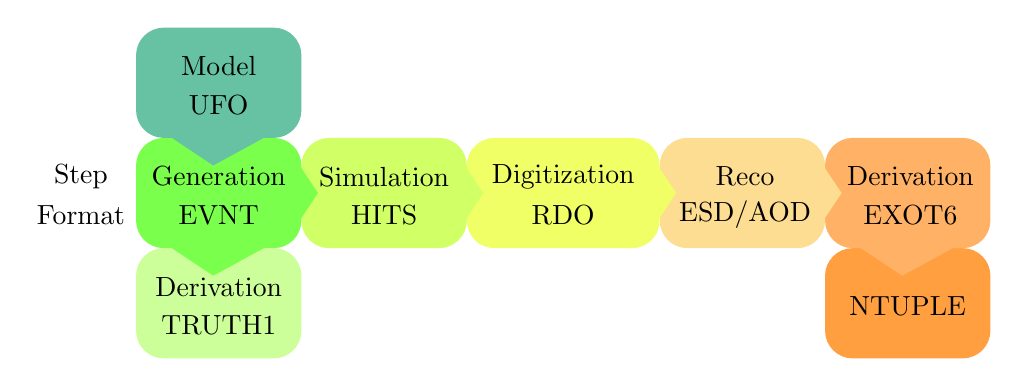
\begin{tikzpicture}[scale=0.7]

	\node[] at (-1,1.3){Step};
 	\node[] at (-1,0.6){Format};
 	
 	\draw[draw=none,fill=orange!75!, rounded corners=10pt] (12.5,0) rectangle +(3,-2);
 	\node[] at (1.5+12.5,-2+0.6+.35){NTUPLE};
 	
	\draw[draw=none,fill=orange!60!, rounded corners=10pt] (12.5,0) rectangle +(3,2);
 	\draw[draw=none,fill=orange!60!] (13,0.1)--(1.4+12.5,-0.5)--(2.5+12.5,0.1) -- cycle;
 	\node[] at (7.75+6.3,1.3){Derivation};
 	\node[] at (7.75+6.3,0.6){EXOT6};
	
	\draw[draw=none,fill=yellow!40!orange!40,rounded corners=10pt] (9.5,0) rectangle +(3,2);
 	\draw[draw=none,fill=yellow!40!orange!40] (12.4,0.4)--(12.8,1)--(12.4,1.6) -- cycle;
 	\node[] at (7.75+3.3,1.3){Reco};
 	\node[] at (7.75+3.3,0.6){ESD/AOD};
	
	\draw[draw=none,fill=green!10!yellow!60,rounded corners=10pt] (6,0) rectangle +(3.5,2);
 	\draw[draw=none,fill=green!10!yellow!60] (9.4,0.4)--(9.8,1)--(9.4,1.6) -- cycle;
 	\node[] at (7.75,1.3){Digitization};
 	\node[] at (7.75,0.6){RDO};
	
	\draw[draw=none,fill=green!30!yellow!60,rounded corners=10pt] (3,0) rectangle +(3,2);
 	\draw[draw=none,fill=green!30!yellow!60] (5.9,0.4)--(6.3,1)--(5.9,1.6) -- cycle;
 	\node[] at (4.5,1.3){Simulation};
 	\node[] at (4.5,0.6){HITS};
 	
 	\draw[draw=none,fill=green!75!yellow!70,rounded corners=10pt] (0,0) rectangle +(3,2);
	\draw[draw=none,fill=green!50!yellow!40,rounded corners=10pt] (0,0) rectangle +(3,-2);
 	\draw[draw=none,fill=green!75!yellow!70] (2.9,0.4)--(3.3,1)--(2.9,1.6) -- cycle;
 	\draw[draw=none,fill=green!75!yellow!70] (.5,0.1)--(1.4,-0.5)--(2.5,0.1) -- cycle;
 	
 	\node[] at (1.5,1.3){Generation};
 	\node[] at (1.5,0.6){EVNT};
 	\node[] at (1.5,-2+1.3){Derivation};
 	\node[] at (1.5,-2+0.6){TRUTH1};
 	
 	\draw[draw=none,fill=green!60!blue!60,rounded corners=10pt] (0,2) rectangle +(3,2);
 	\draw[draw=none,fill=green!60!blue!60] (.5,2.1)--(1.4,1.5)--(2.5,2.1) -- cycle;
 	\node[] at (1.5,3.3){Model};
 	\node[] at (1.5,2.6){UFO};
 	
 	%\node[] at (10.5,1.3){Reconstruction};
 	%\node[] at (10.5,0.6){ESD/AOD};

	%\node[ single arrow , draw, single arrow head extend=.7cm, gray!50, black] at (3.3,0.8) {    };
\end{tikzpicture}
}
\caption{The ATLAS simulation chain. The theoretical model is implemented in a UFO file and given as input to the generation program. Truth level analysis can be pursued, or the EVNT file can be used in a detector simulation whose outcome will be digitized in a RawData Object file and reconstructed in Event Summary Data (ESD) and Analysis Object Data (AOD). A derivation framework runs over the AOD to get the relevant events for a specific analysis. The Derivated Analysis Object Data (DAOD), which in our case is an EXOT6 file, can be made readable by RooT in a NTUPLE form.}
\label{fig:chain}
\end{figure}


\subsection{Generation}
The Minimal model has already been implemented in an UFO file containing its details [cit. al talk di Marta] considering the pure electroweak triplet (\chip\!, \chizero\!, \chim\!) and implemented in FeynRules. Although the model would predict a mass splitting of \SI{166}{\mev} between \chipm and the \chizero, here is set to be \SI{1}{\gev}: small enough to let the charged $\chi$s decay into soft pions and a \chizero but large enough not to create issues in the generation program. 

In this generation process \MGMCatNLO v2.4.0 was used~\cite{madgraph}. This software automatically generates matrix elements as for example decays or scattering from a couple of particles. The user simply specifies the process of interest by giving the initial and final state particles and \MADGRAPH generates the Feynman diagrams and the code needed for the calculation of the matrix element~\cite{Pottgen:2016807}. In this context, even if the software could generate matrix element up to the next to leading order (\NLO) we used only leading order (\LO) calculations. 

Before performing the hadronization and parton shower, a fast scan for different mass point was made in order to get an order of magnitude for the various events cross section. Results are reported in \Tab{\ref{tab:xsectheo}}. The mass used are far below the prediction of the minimal model just because we can't explore the \tev range with LHC \RunTwo data.

\begin{table}[pt]
\centering
\begin{tabular}{ccc}
\toprule
Mass[GeV]&Cross section [pb]&Error [pb]\\
\midrule
\num{1}& \num{0.3069}& \num{0.0020}\\
\num{10}& \num{0.2924}& \num{0.0020}\\
\num{50}& \num{0.01571}& \num{0.00013}\\
\num{100}& \num{4.67e-03 }& \num{0.03e-03}\\
\num{200}& \num{1.164e-03}& \num{0.009e-03}\\
\num{500}& \num{7.54e-05}&\num{0.05e-05}\\
\num{750}& \num{1.369e-05}& \num{0.009e-05}\\
\num{1000}& \num{3.169e-06}& \num{0.021e-06}\\
\bottomrule
\end{tabular}
\caption{Table listing the cross section expected from theory, for several mass points.}
\label{tab:xsectheo}
\end{table}

We generated  \num{10000} events for 21 different $\chi_0$ mass requiring cuts in order to populate the phase space: among other request we demand at least one photon with energy grater than \SI{130}{\gev}.

For the simulation of parton showers, underlying event or hadronization, the output has to be passed on to an external programme, which in our case is \PYTHIA v8.210~\cite{pythia}. This framework accounts for the generation, starting from a \emph{Les Houches Event} (LHE) file, of parton shower and underlying event, i.e. it creates colourless states from free quarks and gluons. \PYTHIA was set up with NNPDF23LO PDF and the A14 tuning. The output file produced is an EVNT file which can be used as input either for the detector simulation step or to produce a TRUTH file.

\subsection{Truth level validation}
\label{sec:truth}
The simulation of the events as it were ``in vacuum'' is called \emph{Truth level}. Here no assumption are made on the detector, but we only want to analyze the process and its outcome. The TRUTH1 is a file coming from a Derivation framework which will be better explained in \Sect{\ref{sec:derivation}}, and it contains all the information we need at this stage.\footnote{Magari potrei spostarlo in fondo al capitolo come derivation alternativa all'EXOT6 fatta al truth level. Cos\`i sono definiti gli oggetti che mi servono per definire i tagli.}

These events are used to define a fiducial region with dedicated selections. It is made to provide useful constraints on new physics which can be re-interpreted in terms of signal models not covered here. The selection involves:
\begin{itemize}
\item photons with $\pt^\gamma>\SI{10}{\GeV}$ with $\abs{\eta_\gamma}<2.37$ and $1.37<\abs{\eta_\gamma}<1.52$;
\item electrons with $\pt^e>\SI{7}{\gev}$ with $\abs{\eta_e}<2.47$;
\item muons with $\pt^\mu>\SI{6}{\gev}$ with $\abs{\eta_\mu}<2.5$\footnote{These last two occurs only for a preselection, no electrons or muons are allowed in this region (see last point)};
\item jets with $\ptjet>\SI{30}{\gev}$ with $\abs{\eta_{\textup{jet}}}<4.5$ not overlapping with electron or photon by $\DeltaR > 0.4$;
\item $\met>\SI{150}{\gev}$;
\item leading photon with $\pt^\gamma > \SI{150}{\GeV}$;
\item \met significance: $\met/\sqrt{\sumET} > \SI{8.5}{\GeV^{1/2}}$;
\item no electrons nor muons and $N_\textup{jets}\le 1$ with $\Delta\phi_\textup{jet-\met}<0.4$ if any.
\end{itemize}


Now, from several TRUTH files for different masses, we would like to validate the sample and check the kinematics. The results are stored in validation plots in \Fig{\ref{fig:validation}}. In these plots for different DM masses. Notice that the peak for low-$\pt^\gamma$ in \Fig{\ref{subfig:phpt}} rises because the leading photon could get in the crack region (\etaRange{1.37}{1.52}) and therefore doesn't pass the $\eta$ cuts. Then the code select a subleading photon with lower momentum\footnote{A weird behaviour has been noticed in \PYTHIA for which sometimes the leading photon converts in a couple $e^+e^-$ for apparently no reasons. These events, however, contribute to the sharp low peak but they occur in the 5\% of the case and they can be neglected}. Detailed analyisis on these events in terms of fiducial cross section will be given {\bfseries in the next chaplter}.

\begin{figure}[t]
\centering
\subfloat[][Photon momentum for different masses. \label{subfig:phpt}]
{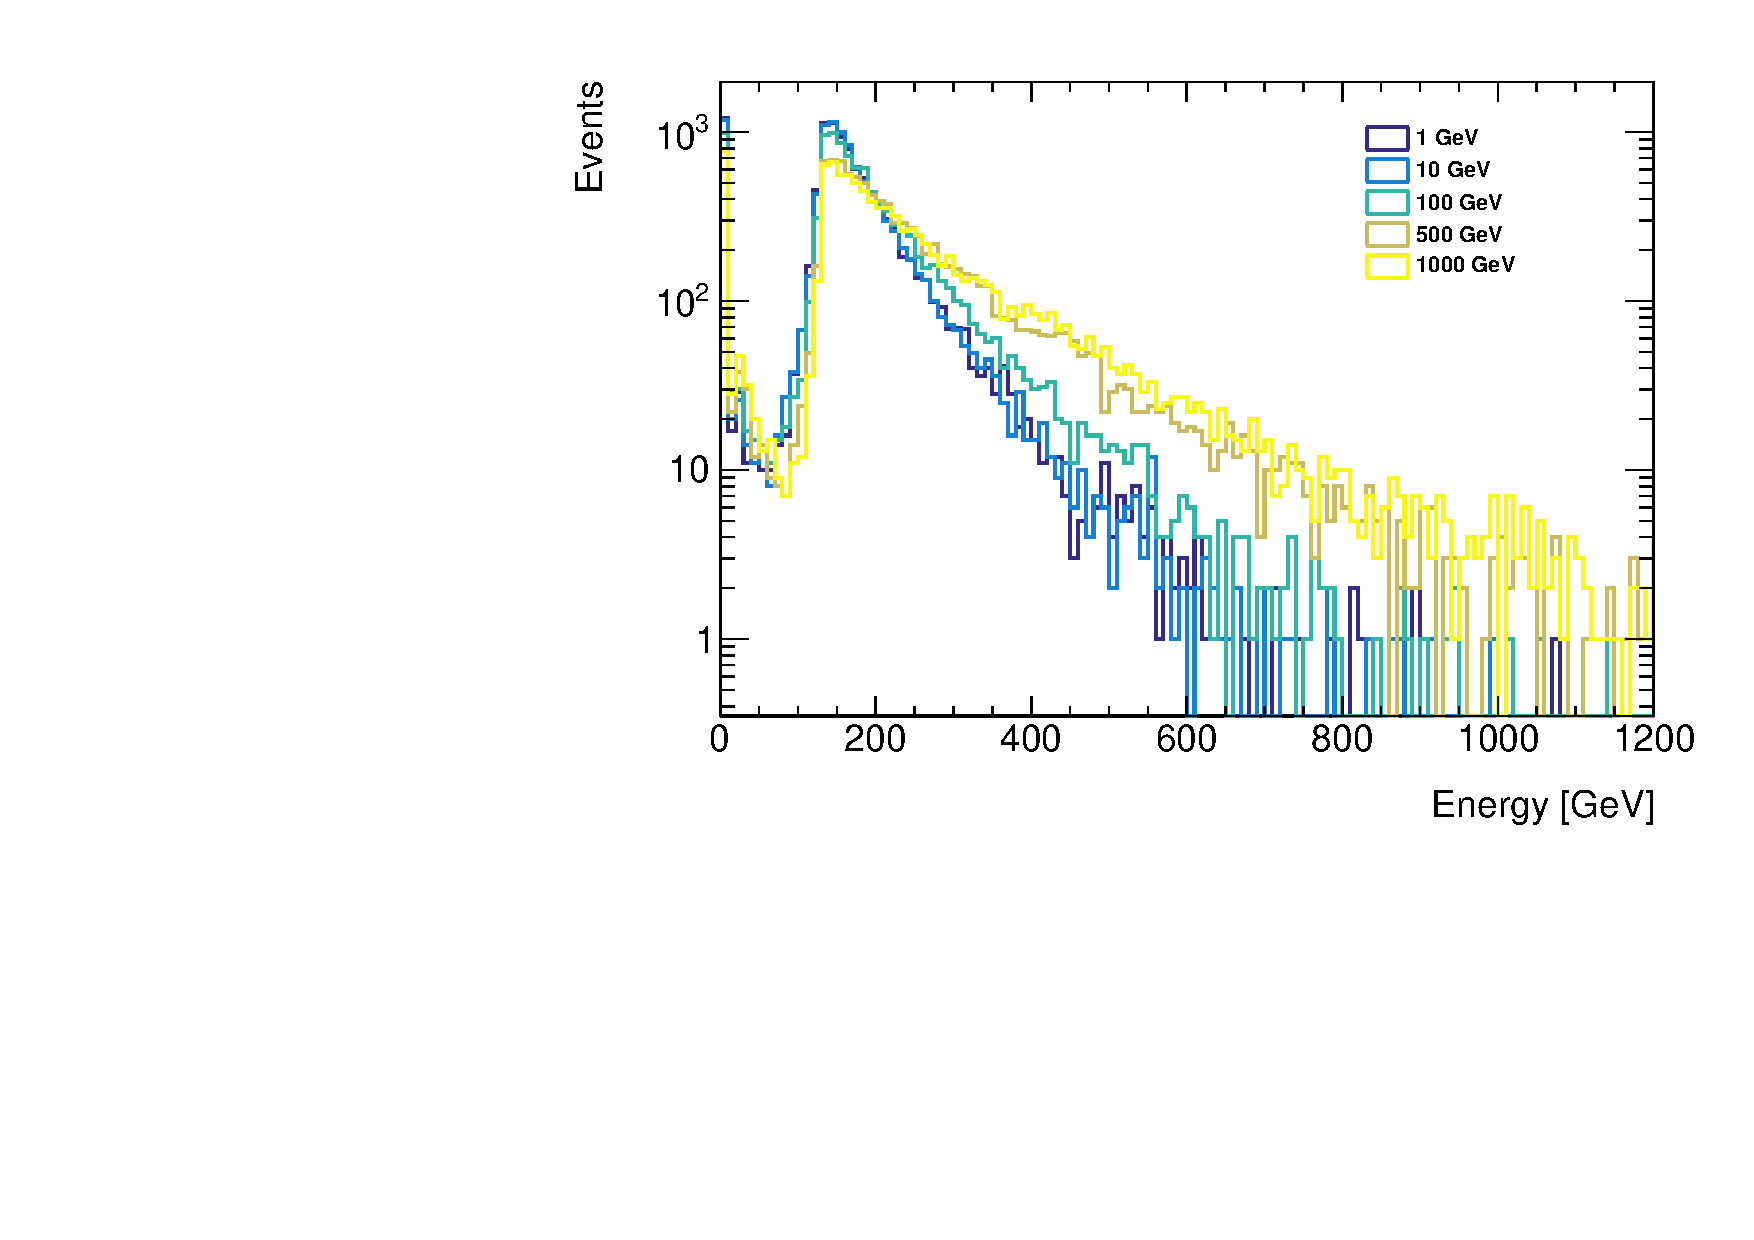
\includegraphics[width=.45\textwidth]{MCSample/canPhPtoverlap}} \quad
\subfloat[][Missing energy for different masses]
{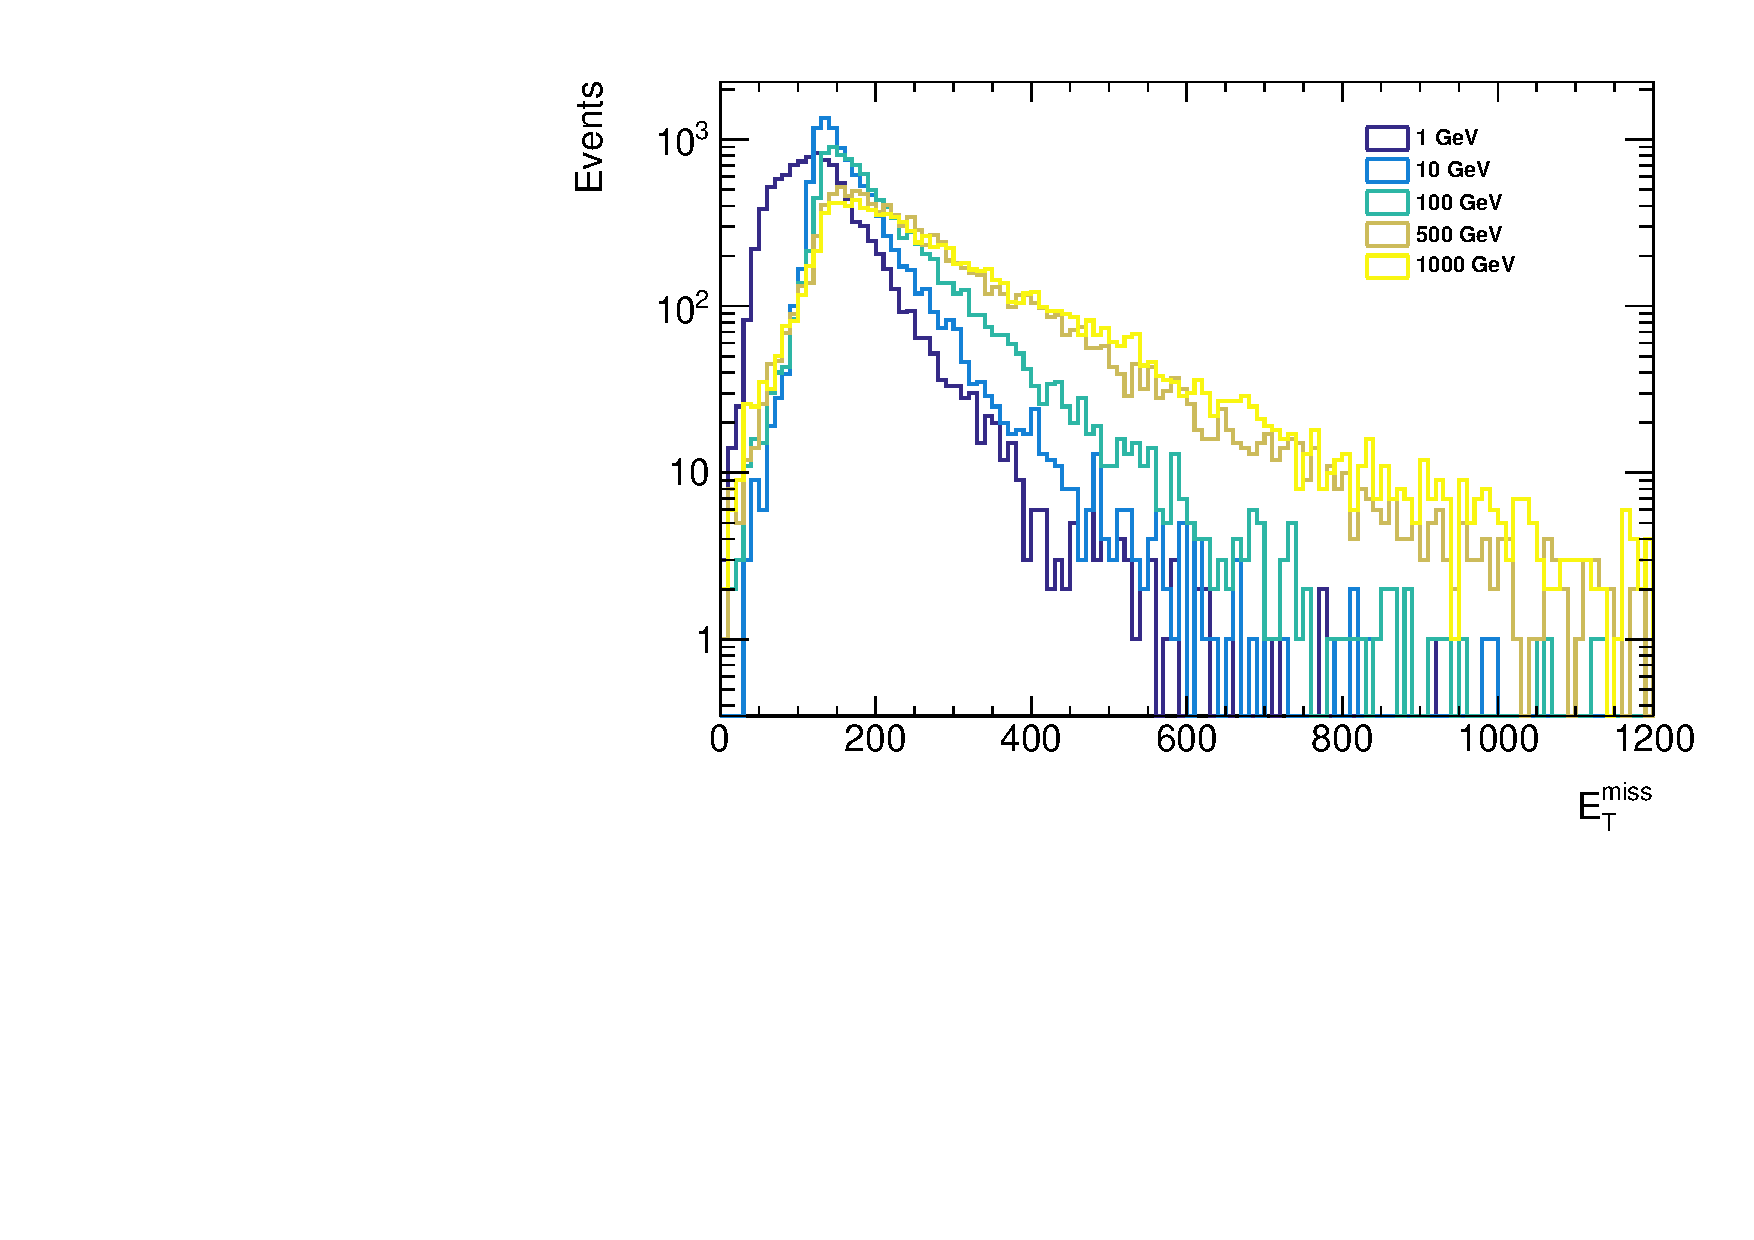
\includegraphics[width=.45\textwidth]{MCSample/canMEToverlap}} \quad
\subfloat[][Pseudorapidity of the photon for different masses]
{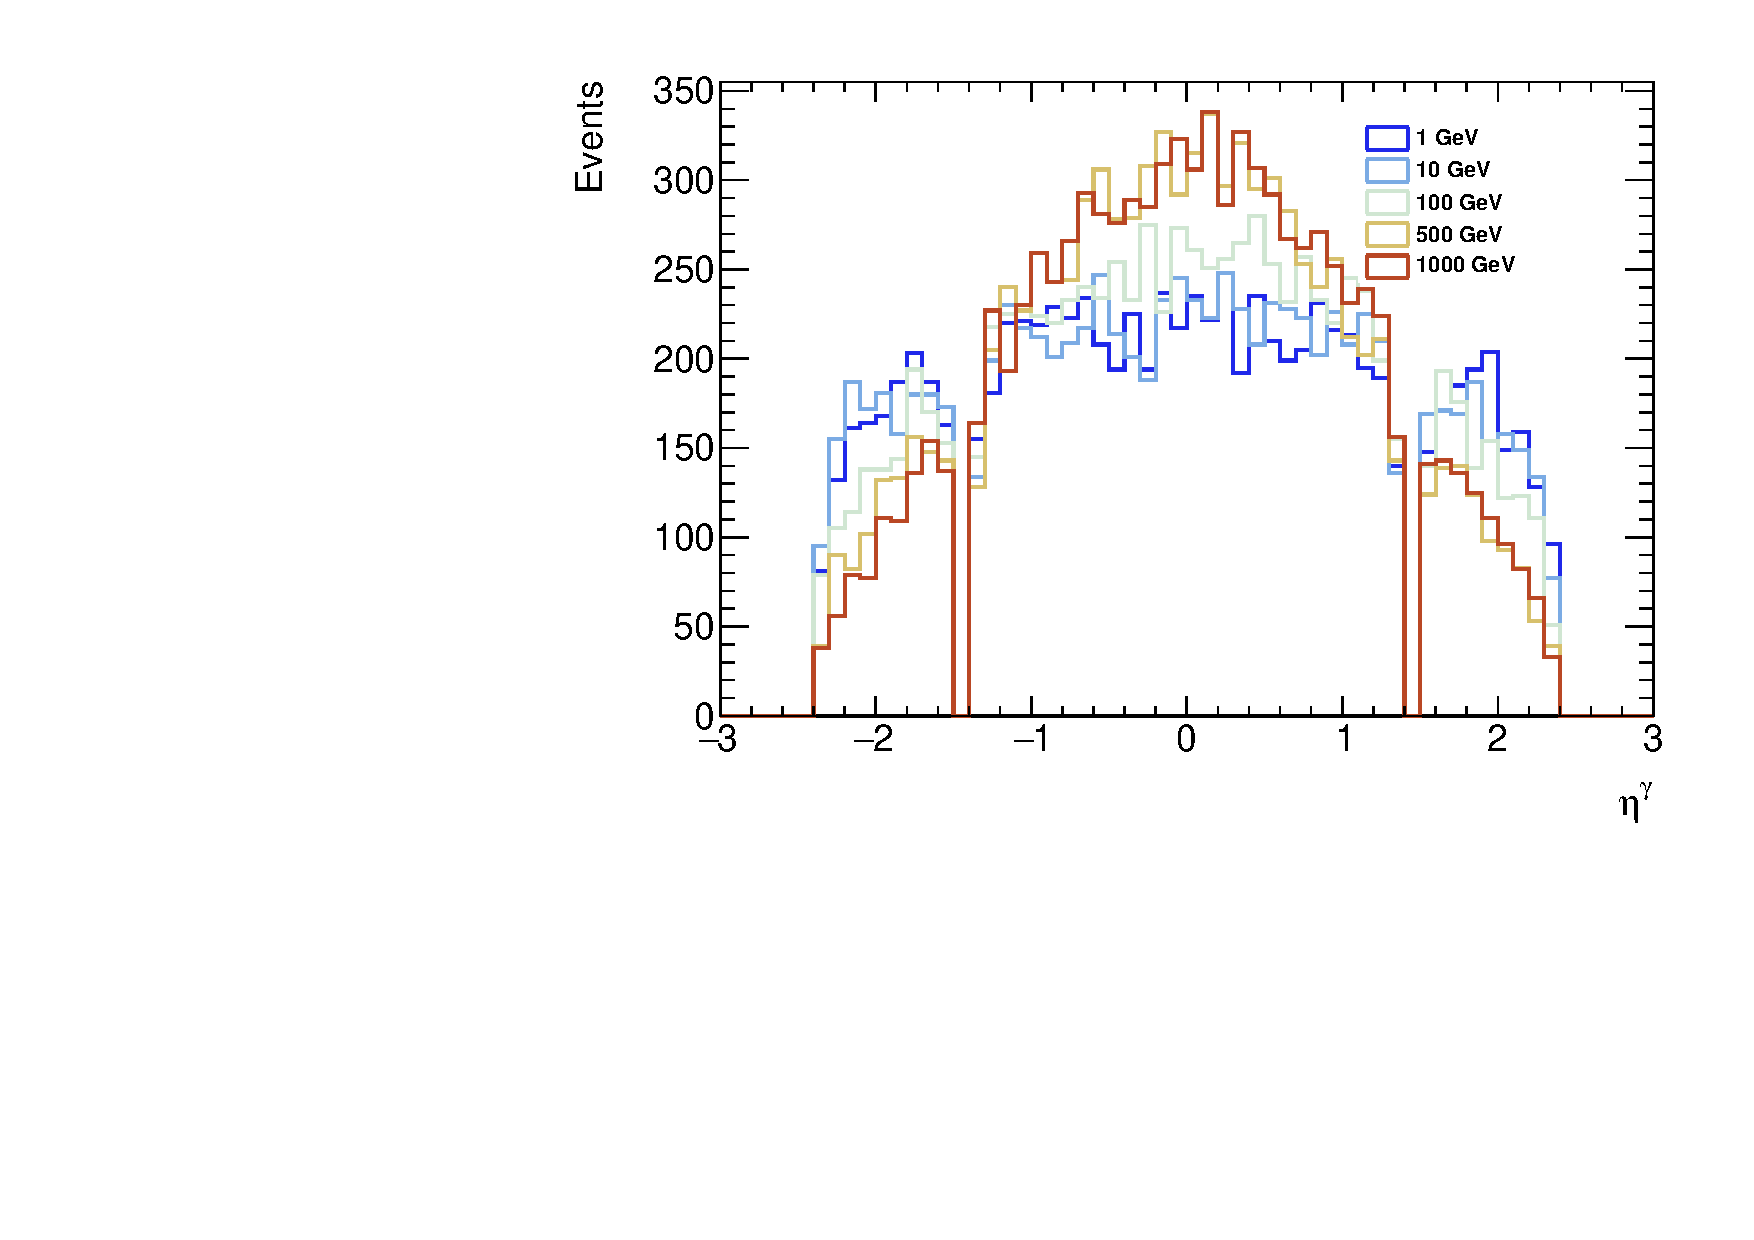
\includegraphics[width=.45\textwidth]{MCSample/canEtaoverlap}} \quad
\subfloat[][Number of jets for different masses]
{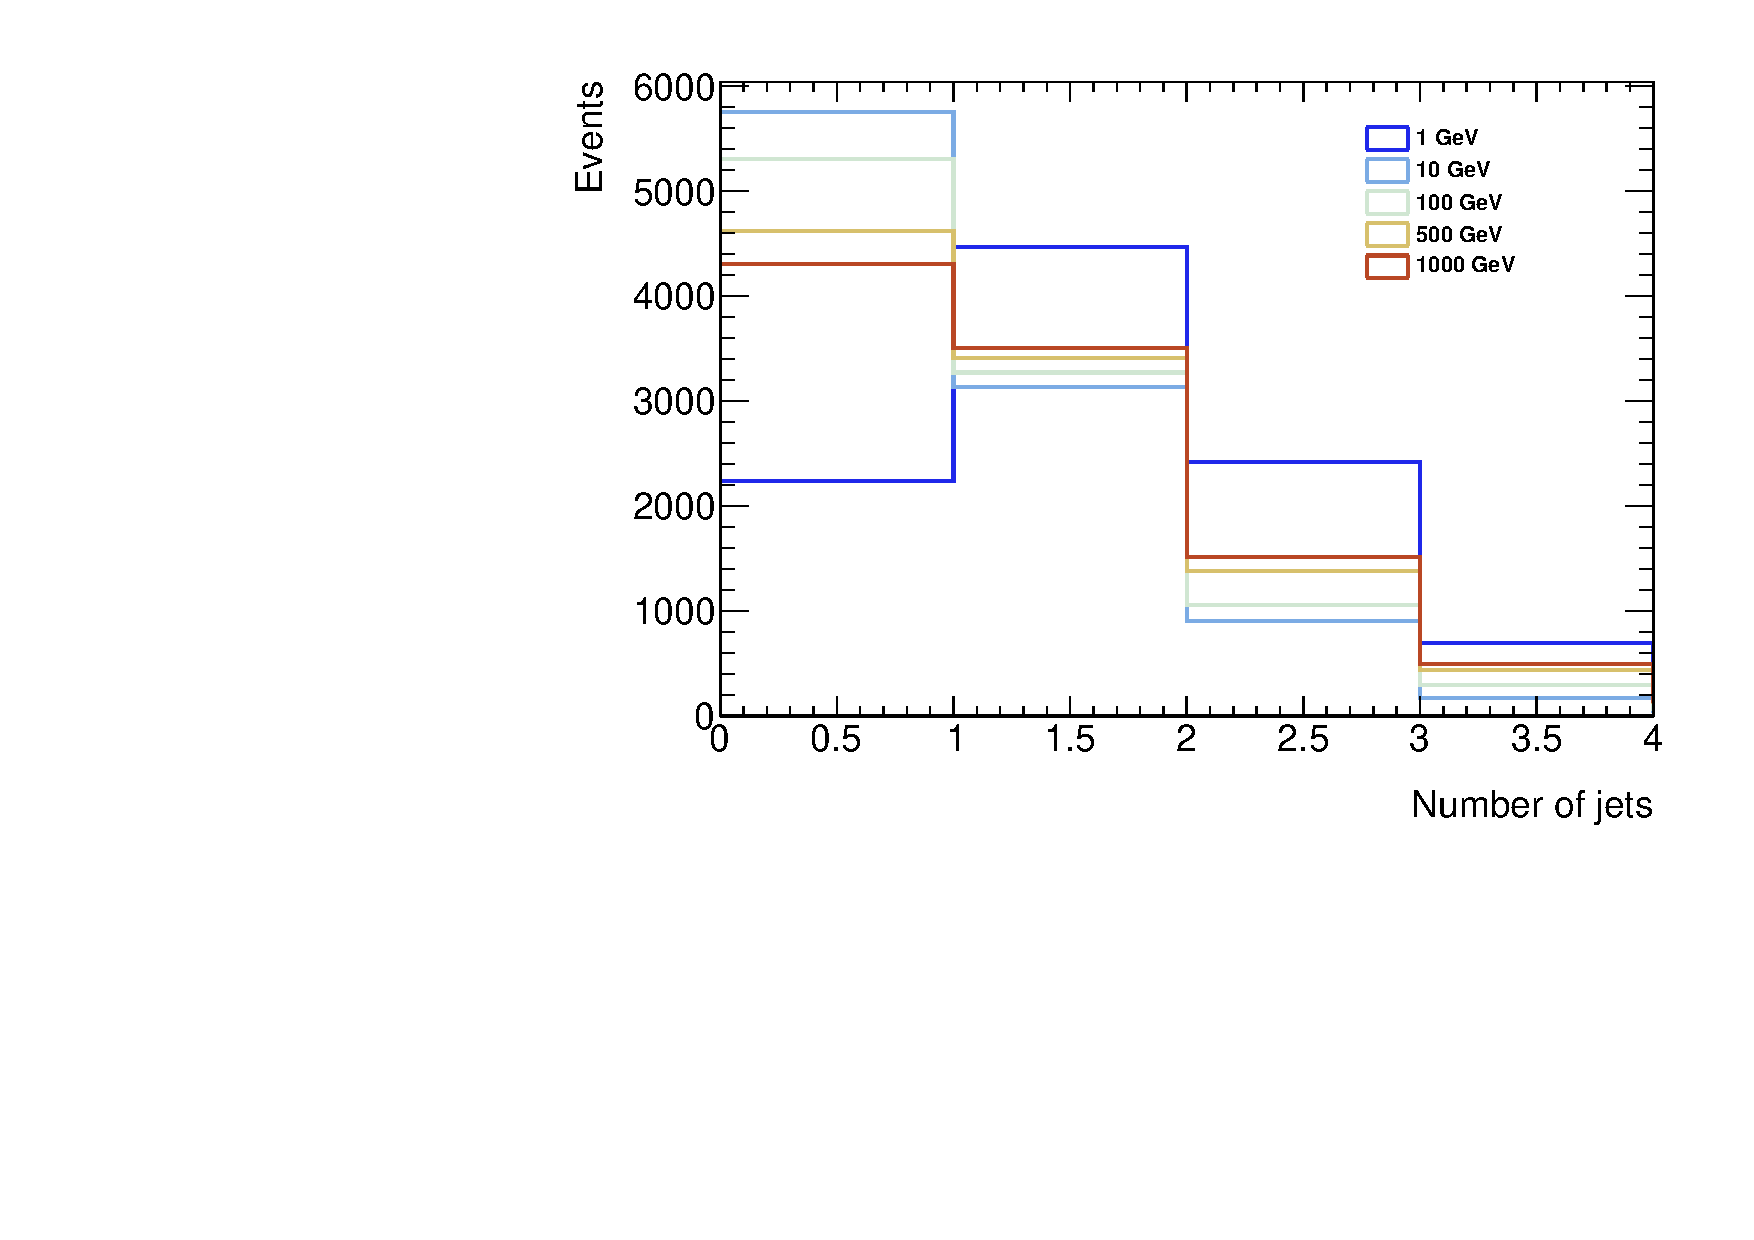
\includegraphics[width=.45\textwidth]{MCSample/canNjetsoverlap}} \quad
\caption{Validation plots for the Minimal DM model. From these plots an evolution on kinematics variables can be seen as a function of DM mass.}
\label{fig:validation}
\end{figure}

\subsection{Simulation}
The standard simulation of ATLAS relies on the \geant particle simulation toolkit which is a toolkit for simulating the passage of particles through matter. This step takes as inpunt the EVNT file from \PYTHIA, in our case, or any of the generators such \HERWIG and \SHERPA, and it is the most time expensive stage in the full simulation. The output is stored into an HIT file. To save time the framework allows the user to skip a certain number of events at the beginning of an input file by submitting $n$ jobs with $N$ events each to a $n\times N$ event input file and merged together at the end of the process.

%First of all comes the simulation initialization which is divided in three steps. Stage one of the initialization occurs as soon as Athena is started which is set to AtlasProduction 19.2.4.9. release. Here job properties provided by the user are locked, metadata that will be stored with the hit output file are gathered and the HIT file initialized. Finally service is created to interface with \geant which is not fully initialized at this stage. In stage two detector, physics regions, range cuts are created. Each piece of the ATLAS detector is constructed in GeoModel according to the geometry chosen, which in this work is \verb!ATLAS-R2-2015-03-01-00_VALIDATION!, and translated into an equivalent \geant geometry. Next, the Monte Carlo truth strategies, which are \verb!MC12! in this context, are added to the simulation.Then the magnetic field is loaded and every user action, which allows a user to insert pieces of code in various places throughout the simulation event loop, provided from the configuration command are initialized. The physics list (see below) used for simulation is also set at this point. The third stage completes the job preparation. assigning fast simulation models and runs \geant  software.

%A physics list contains all numerical models that describe the particles' interactions in the \geant simulation. The \geant Collaboration provides several combinations of these models for every possible physical outline. We used the \verb!FTFP_BERT! phisics list which is the current \geant default. Any further information can be found in~\cite{ftfpbert}.

To speed up the process that could get very long in time is to approach the Fast Simulation. In this work ATLFAST-II was used. ATLFAST-II is a fast simulation which provides large statistics to supplement full simulation studies. It is made up from two components: the Fast ATLAS Tracking Simulation (Fatras) for the inner detector and muon system simulation and the Fast calorimeter Simulation (FastCaloSim) for the calorimeter simulation. 

In Fatras for the geometry of the detector is a simplified description of the full detector geometry which manains the same descriptive accuracy for its sensitive parts, and all other detector components are approximated as simplified layers that carry a high-granularity density providing an improvement in CPU time by a factor \num{100}. The interactions of the particles with the simplified detector layers are simulated using several methods, for instance ionization and radiative energy loss are simulated according to the Bethe-Bloch model, the photon conversion into a couple electron and positron is performed depending on the thickness of the material crossed and hadronic interactions with the detector layer are simulated from a parametric model obtained from \geant simulation results. Fatras provides also the input particle collection to give to FastCaloSim. Moreover it records energy deposition for muons in the calorimeter layers which will be used in the FastCaloSim application. The trajectories of the muons are also simulated in the muon spectrometer.

FastCaloSim uses parametrizations of the longitudinal and lateral energy profile of the energy of single particle showers instead of simulating the particle interactions with the detector material. The parametrizations are based on a fully-simulated, with \geant, sample of 30 million events made of single photons and charged pions from an energy range between \SI{200}{\MeV} and \SI{500}{\GeV} for \AetaRange{5.0} and every $\phi$. Electron and photon showers are approximated by the photon parametrization and hadronic showers are modeled on the charged pions.

The output from the simulation is a HITS file. The hits are records of energy deposition, with position and time, during the simulation. Most of them comes from the Inner Detector for which the majority of hits are independently stored and occupying about \SI{1360}{kB} per event while the muon system collects far fewer hits than the other subsystems and requires less disk space for the hit records (\SI{\sim3}{kB\per event}).

In order to understand anomalies and debug errors due to geometry or checking by eye overlaps and touching volumes in geometry a visualization step could also be performed. An examples of events are shown in \Fig{\ref{fig:simulation}}.

\begin{figure}[tp]
\centering
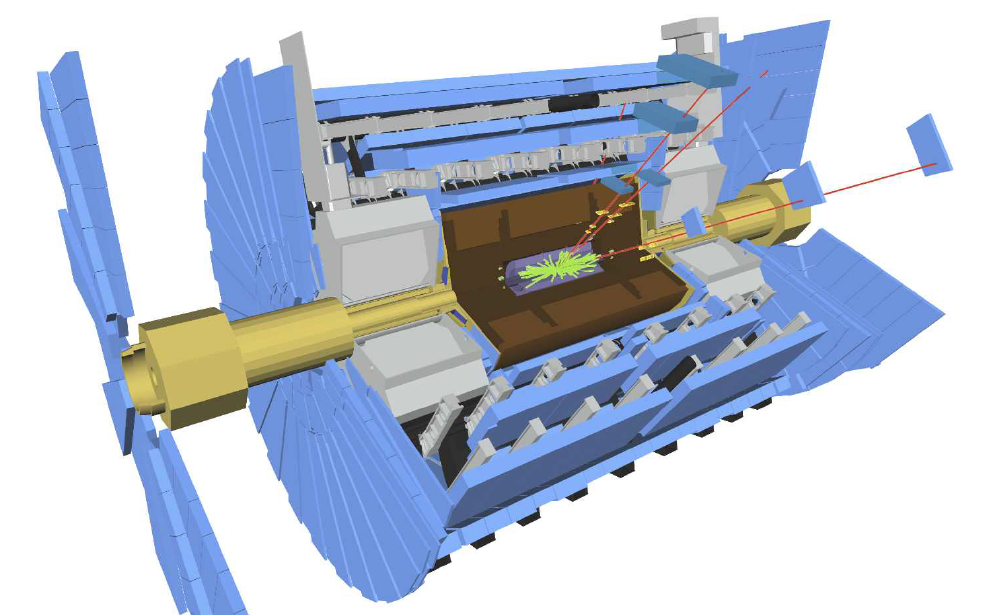
\includegraphics[width=.75\textwidth]{MCSample/simulation}
\caption{An event display made with VP1. VP1 is a viewing software made specifically for ATLAS which stands for Virtual Point 1, since ATLAS is situated at Point 1 of the LHC ring. It shows a Higgs boson decaying into four muons (shown in red). Inner detector tracks are in green, and energy deposited in the calorimeter by the muons is shown in yellow.}
\label{fig:simulation}
\end{figure}

\subsection{Digitization}
The ATLAS digitization software converts the hits produced by the core simulation into detector responses i.e ``digits''. In real events a digit is produced when the voltage of a readout channel rises above a preconfigured threshold in a particular time window.

{\bfseries ora inizia parte poco chiara, perch\'e il paper parla solo di hard scattering digitizzato. non c'era tutto nel file hit?}

In addition to the hard scattering digitization pile-up and any other source of noise must be incorporated. For pile-up simulation, there are also input HIT files for each type of background interaction to be overlaid. whose number for each bunch crossing is a function of the luminosity simulated. Moreover cavern background could influence the simulation. The cavern background is a sort of neutron-photon gas made up from neutrons propagating into the ATLAS cavern before getting thermalized. 

The ATLAS detector electronics produce data in bytestream format called RawData Objects (RDO) whose size on disk is typically \SI{2.5}{MB\per event} and increases with larger number of \pileup.

RDO TRIGGER?

\subsection{Reconstruction}
\'E la stessa cosa che accade con oggetti reali? Va bene se qui metto quello che poi scriver\'o pi\'u avanti Nell1 1.4?

\subsection{EXOT6 Derivation}
During \RunTwo ATLAS, by proposal by the Analysis Model Study Group (AMSG), has developed a ``derivation framework'' which works on the principle that analysts need to be able to run over their data sample frequently. For this purpose the derivation framework provides the offline software tools and structures to work on data in a very simple way. 

Unlike in \RunOne when derivation was made by users, this production is now made centrally by the ATLAS production services, even if it can be run locally as in our case, avoiding difficulties in cross-team analyses due to differences in the formats and in reading the output file.

Derivations will be made from the full data via four operations:
\begin{enumerate}
\item skimming: the removal of the entire event,
\item thinning: when removing the whole objects in an event, but keeping the rest of it,
\item slimming: information removal from objects, while keeping the rest of it,
\item augmentation: adding data not found in the input data.
\end{enumerate}

Therefore the derivation framework selects only the relevant data for a specific analysis, from all ATLAS data collected. This functioning is well explained in the sketch shown in \Fig{\ref{fig:derivation}}.

For this analysis a specifix derivation called ``EXOT6'' has been implemented and the following skimming selection was applied:
\begin{itemize}
\item Event must pass one out of several trigger request, including the \verb!HLT_g140_loose! which this analysis is based on;
\item Event must have one loose\footnote{see \Sect{\ref{photons}}} photon with $\pt\ge\SI{80}{\gev}$ or one loose electron with $\pt\ge\SI{100}{\gev}$.
\end{itemize}
\label{sec:derivation}

\begin{figure}[tp]
\centering
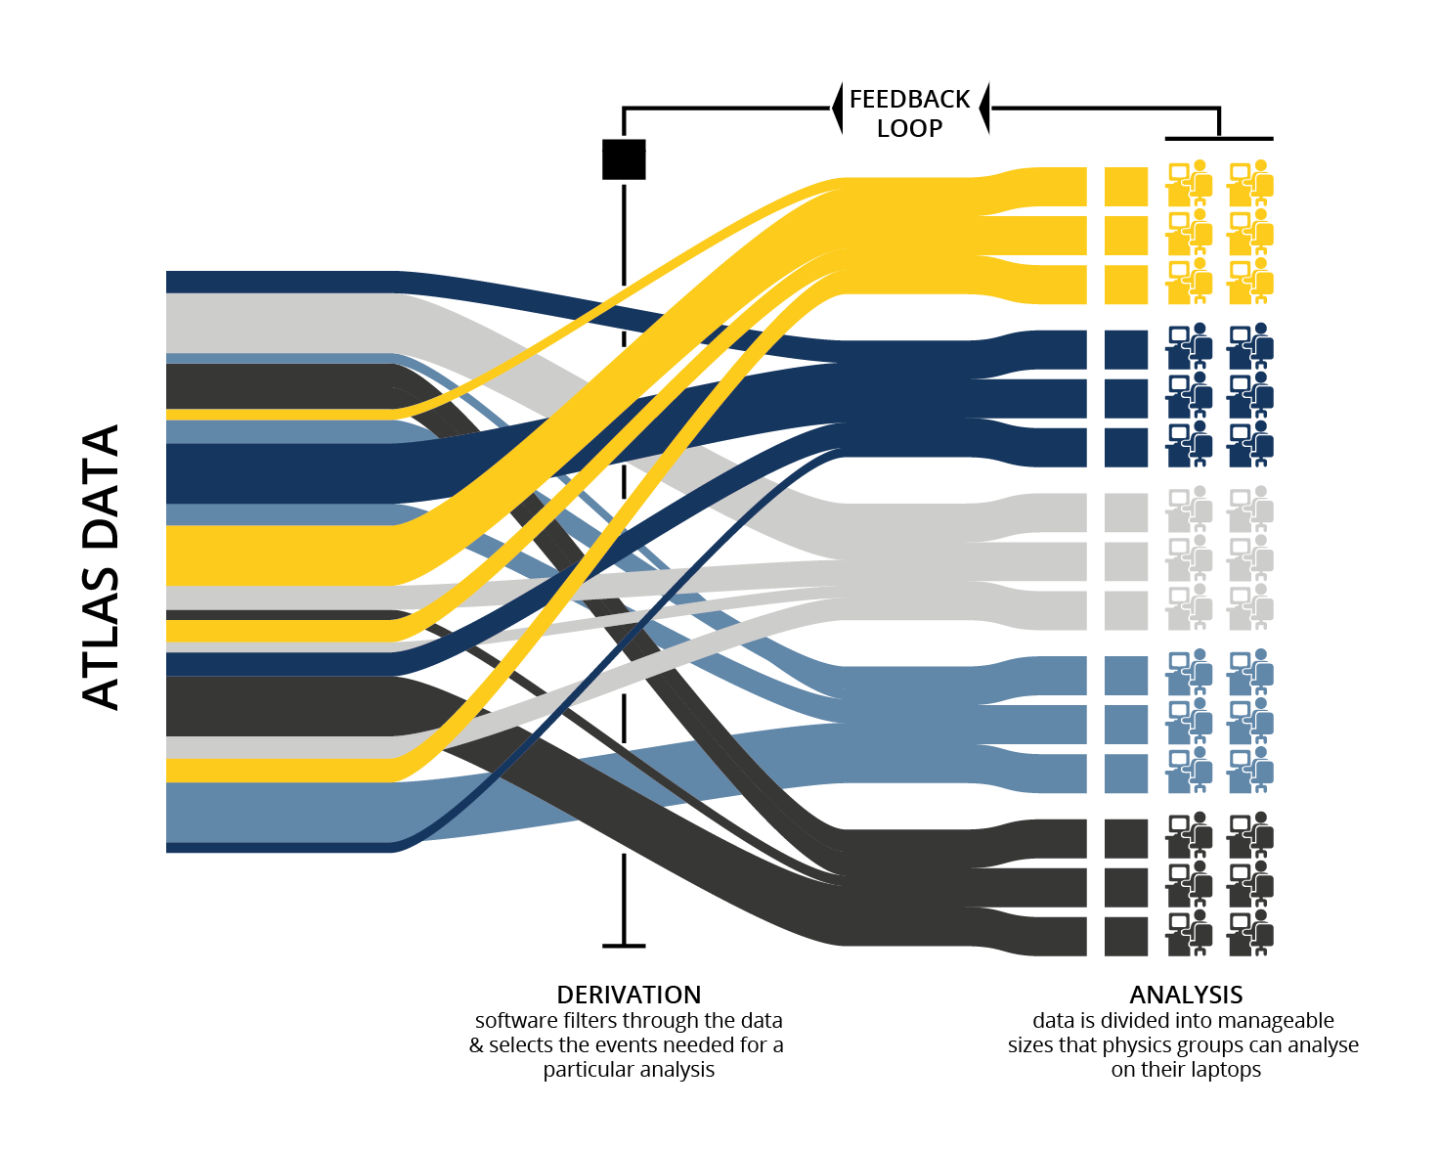
\includegraphics[width=.7\textwidth]{MCSample/Derivation}
\caption{Sketch of how the derivation code works for ATLAS data. Each single event from the whole amount of ATLAS data contains different characteristics that the derivation code depending on the analysis performed.}
\label{fig:derivation}
\end{figure}

DICO QUALCOSA ANCHE SULLA GENERAZIONE DEI MINITREE?

\section{Piccolo recap}
Se ho capito bene, dalla digitizzazione in poi il processo per MC e dati reali \`e lo stesso. Solo la simulazione del rivelatore, ovvio, \`e fatta per i MC.
Il dubbio rimane sulla reco: \`e la stessa? Cio\`e la ricostruzione avviene allo stesso modo?

\section{Reconstruction of real objects in ATLAS}
\label{sec:recoreal}
Within this section, real object definition and reconstruction in ATLAS is given, focusing on those which this analysis holds togheter. Definitions follows the recommendations from the various combined performance groups. 

An evente in ATLAS is an ensemble of signal produced in the detector which must be processed in order to get particle's property and identification. 

\subsection{Photons}
\label{photons}
\subsubsection{Reconstruction}
Photons are reconstructed from clusters in the electromagnetic calorimeter measured in projective towers but uses information from the Inner Detector as well. These towers are portion of the second layer of the calorimeter of $N_1 \times N_2$ cells in the $\eta-\phi$ plane. Photons and electrons (positrons) signature and energy deposits are very similar in the EM calorimeter. That's why we need information from ID to discriminate them: a photon would not produce any tracks there since the ID is sensitive only to charged particles. A cluster with no tracks associated is therefore a photon which is defined \emph{unconverted} since after it was produced in a primary vertex it is straight revealed by the EM calorimeter. A \emph{converted} photon, instead, is produced in a primary vertex, it generats a electron-positron couple in a secondary vertex within the ID and in the calorimeter it produces two associated tracks.

The reconstruction process starts from a \emph{sliding-window} algorithm. It looks for the optimal clusters starting from windows of $3\times5$ cells, or $0.025\times0.025$ in $\eta-\phi$, for unconverted photons and $3\times7$ cells ($0.175\times0.175 \, \eta\times\phi$) for converted ones, in the barrel region of the EM calorimeter, whose energy deposited is greater than \SI{2.5}{\gev} in order to reduce electronic noises and any \pileup events. In the endcap, clusters of size $5\times5$ are used for all photon candidates.

In order to identify an object as a photon or electron tracks information are necessary. The tracking algorithm, Gaussian Sum Filter (GSF), reconstructs tracks by fitting points within the pixel detector and first layers of SCT and extrapolates informations gathered to outer layer of the ID and into the EM calorimeter. The algorithm also carefully trets the energy losses due to bremsstrahlung. Working along with the tracking algorithm, the vertexing algorithm analyses and classifies the interaction verteces and requires that a track points toward the center of the cluster whithin a $0.05\times0.05$ $\eta\times\phi$ window. Clusters with no matching tracks are classified as unconverted photons. Otherwise it is reconstructed as a converted photon or an electron.

Any noisy or sporadic noisy channel can sometimes produce a signal with transverse momentum larger than \SI{2.5}{\GeV }and give rise to a sliding window cluster~\cite{photons}. In order to identify these bad quality or fake clusters coming from instrumental problems cleaning cuts are applied on photon candidates. A photon is flagged as bad if it contains or edges dead/masked cells.

\subsubsection{Identification}
Once a list of candidate photons has been made, we have to discriminate between real photons and contamination from \pizero, as shown in \Fig{\ref{pizerogamma}}, or other SM particles decaying via two photons. Identification is based upon the strip and middle layers of the EM calorimeter.

Two working point are defined for photons: loose and tight depending on which cuts a photon passes based on shower shapes measured in strips and middle layers of the EM calorimeter together with hadronic leakage. The differences observed between data and MC in the ``isEM'' discriminating variables are measured comparing the shower shape distributions, and parametrized as simple shifts.{\bfseries POCO CHIARO}. Instead, three working points which are loose, medium and tight, have been defined for electrons. Details on photons selection criteria can be found in \cite[Sect. 4]{photons}.

\subsubsection{Isolation}
\begin{figure}[tp]
\centering
\subfloat[scale=1.5][\label{pizerogamma}]
{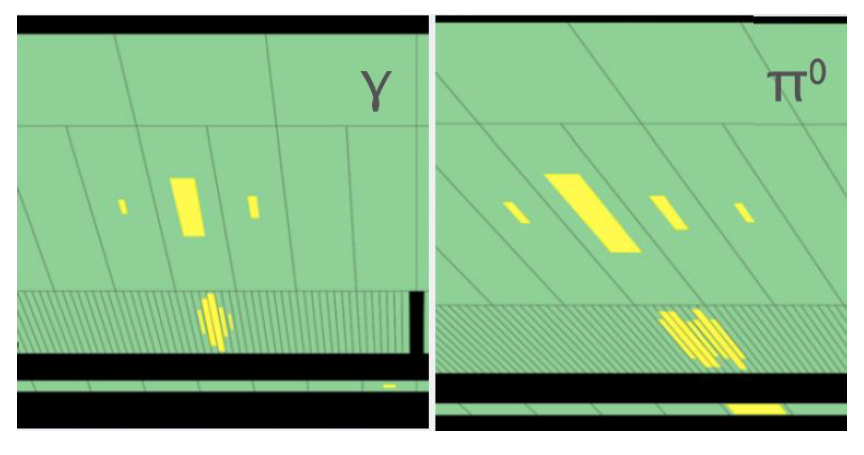
\includegraphics[width=.45\textwidth]{MCSample/pizerogamma}} \quad
\subfloat[0.4\textwidth][\label{topoetcone40}]
{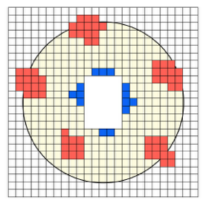
\includegraphics[scale=0.6]{MCSample/topoetcone40}} 
\caption{(\emph{a}). Discrimination between a single photon and two collimated photons from a \pizero decay in the the ATLAS EM calorimeter. From the bottom to the top the strip, middle and back layers are visualized. \\ \emph({b}). The algorithm which fills TopoEtCone40 in action: from the $R=0.4$ cone (yellow) a $5\times7$ rectangle is removed, energy deposited is computed among the \topo~within the cone (orange) and the \pt-leakage (blue) is subtracted.}
\end{figure}
Usually the isolation of a particle is expressed in terms of $E_\textup{T}^{\textup{iso}}$ which computes the transverse energy of the calorimeter cells (\topo) whithin a cone of given radius around a candidate. A track isolation $p_\textup{T}^{\textup{iso}}$variable can be defined as well.

In the above mentioned cone, an algorithm looks for \topo~with energy deposits above a certain threshold. If any has been found, the contribute of the photon itself, in a $5\times7$ cells area around the cone axis, and from the underlying evens and \pileup is therefore subtracted and the \pt-leakage, i.e. photon energy escaped frome the area previously identified, is taken into account. Then the total energy in the cone is computed and the variable storing this information in our analysis is ``TopoEtCone40'' which contains the energy evaluated in a cone of $R=0.4$ radius. Therefore a photon is considered isolated if ``TopoEtCone40''remains below a certain threshold, i.e. $\text{TopoEtcone40} < 0.022\pt^\gamma + \SI{2.45}{\GeV}$ and $\text{ptcone20}/\pt^\gamma<0.05$. A visual representation of the process described is given in \Fig{\ref{topoetcone40}}.

All the reconstructed loose photons with \ET $> \SI{10}{\GeV}$ (after energy rescaling) and $\eta<2.37$ are considered as photon candidates.


\subsection{Missing transverse momentum}
\subsubsection{Reconstruction}

An intuitive definition of missing transverse momentum (\met) is the momentum inbalance in the transverse plane. A non-zero inbalance there, must suggest the presence of missing energy since this plane is boost-invariant and energy must be conserved. Indeed we can state something only about this energy since any beam-projected component could carry a fraction of proton momentum at which the collision took place, which is unknown\footnote{boh, magari l'inglese \`e sbagliato. Cio\`e voglio dire che non conosciamo l'energia longitudinale perch\`e il momento del partone \`e ignoto, ma l'energia del piano trasverso \`e nulla e tale deve rimanere}.

\met could be given simply by neutrinos, malfunctioning in the detector or its finite resolution so that a reconstructable particle becomes invisible or it could be relevant for this analysis for which it stands to \emph{non}-interacting particles such DM particles.

Here we refer to the scalar quantity with \met and to the vectorial with \textbf{\met}. For a detailed approach to the calibration and reconstruction of this quantity refer to \cite{met}.

The \met calculation used in this analysis is based on reconstructed and calibrated physics objects. In the transverse plane the scalar energy and the corresponing vector quantity are given by:
\begin{gather}
\label{eqn:met}
	\met=\sqrt{(E_x^\textup{miss})^2+(E_y^\textup{miss})^2}\\
	\textbf{\met}=\met \hat{n}
\end{gather}

where $\hat{n}$ is a versor pointing from the origin of the ATLAS reference frame toward the direction in which \met is found.

The single components $E_i^\textup{miss}$, ($i=\{x,y\}$), in equation \ref{eqn:met} is given by:
\begin{equation}
	E_i^\textup{miss}=E_i^\textup{miss,$e$}+E_i^\textup{miss,$\gamma$}+E_i^\textup{miss,$\mu$}+E_i^\textup{miss,$\tau$}+E_i^\textup{miss,jets}+E_i^\textup{miss,Soft}
\end{equation}

Each term is calculated as the negative sum of the reconstructed objects, projected on the transverse plane and reverting the corresponding \pt. The ``Soft'' term is calculated from energy deposits or tracks which are not matched to selected hard objects. 

There are several computation of \met. The one upon this analysis is based is the ``Track Soft Term'' (TST) calculated from the tracks from the primary vertex that are not matched to selected hard objetcs providing a stronger measurement against pileup~\cite{Brunt:2013489}.













